% =========================================================
%  Sapienza Università di Roma  Beamer Presentation
%  Non-reciprocal Effects in 2D Superconductors
%  studied by Conformal Mapping
%  Francesco Lupicuti | A.Y. 2025/2026
% =========================================================
\documentclass[aspectratio=169, 10pt]{beamer}

\usepackage[utf8]{inputenc}
\usepackage[T1]{fontenc}
\usepackage[english]{babel}
\usepackage{lmodern}
\usepackage{microtype}
\usepackage{amsmath, amsfonts, amssymb}
\usepackage{physics}
\usepackage{graphicx}
\usepackage{tikz}
\usetikzlibrary{calc, shapes.geometric, arrows.meta}
\usepackage{xcolor}
\usepackage{tcolorbox}
\tcbuselibrary{skins, breakable, xparse}
\usepackage{appendixnumberbeamer}

% ===========================================================
%  COLOUR PALETTE
% ===========================================================
\definecolor{SapienzaRed}{HTML}{822433}
\definecolor{SapienzaDark}{HTML}{4A0E17}
\definecolor{SapienzaGold}{HTML}{A87C2A}
\definecolor{SlateGray}{HTML}{2E3440}
\definecolor{LightGray}{HTML}{F0F0F0}
\definecolor{MidGray}{HTML}{888888}
\definecolor{AccentBlue}{HTML}{2E5F8A}

% ===========================================================
%  CUSTOM MINIMAL THEME
% ===========================================================
\usetheme{default}
\setbeamercolor{background canvas}{bg=white}
\setbeamerfont{frametitle}{series=\bfseries, size=\large}

%  Frametitle: red bar + gold line â€â€Â
\setbeamercolor{frametitle}{bg=SapienzaRed, fg=white}
\setbeamercolor{frametitle gold rule}{bg=SapienzaGold}
\setbeamertemplate{frametitle}{%
  \nointerlineskip
  \begin{beamercolorbox}[wd=\paperwidth, ht=0.62cm, dp=0.10cm,
        leftskip=0.5cm, rightskip=0.3cm]{frametitle}
    \vskip3pt\usebeamerfont{frametitle}\insertframetitle\vskip3pt
  \end{beamercolorbox}%
  \nointerlineskip
  \begin{beamercolorbox}[wd=\paperwidth, ht=1.5pt, dp=0pt]{frametitle gold rule}{}%
  \end{beamercolorbox}%
}

%  No headline â€â€Â
\setbeamertemplate{headline}{}

%  Footer â€â€Â
\setbeamertemplate{navigation symbols}{}
\setbeamercolor{footline bar}{bg=SapienzaRed, fg=white}
\setbeamertemplate{footline}{%
  \begin{beamercolorbox}[wd=\paperwidth, ht=0.38cm, dp=0.10cm,
        leftskip=0.4cm, rightskip=0.4cm]{footline bar}%
    \textcolor{white!70}{F.\ Lupicuti}%
    \hfill
    \textcolor{white}{Non-reciprocal Effects in 2D Superconductors}%
    \hfill
    \textcolor{white!70}{\insertframenumber\,/\,\inserttotalframenumber}%
  \end{beamercolorbox}%
}

%  Items & Lists (Beamer-Native Spacing) â€â€Â
\setbeamertemplate{itemize item}{\textcolor{SapienzaRed}{\small$\blacksquare$}}
\setbeamertemplate{itemize subitem}{\textcolor{SapienzaGold}{\small$\bullet$}}
\setbeamertemplate{enumerate item}{\textcolor{SapienzaRed}{\bfseries\insertenumlabel.}}

\addtobeamertemplate{itemize/enumerate body}{\setlength{\itemsep}{1pt}\setlength{\topsep}{1pt}\setlength{\parsep}{0pt}\setlength{\partopsep}{0pt}}{}
\addtobeamertemplate{itemize/enumerate subbody}{\setlength{\itemsep}{1pt}\setlength{\topsep}{1pt}\setlength{\parsep}{0pt}\setlength{\partopsep}{0pt}}{}

% Global spacing
\setlength{\parskip}{0pt}
\setlength{\abovedisplayskip}{2pt}
\setlength{\belowdisplayskip}{2pt}
\setlength{\abovedisplayshortskip}{1pt}
\setlength{\belowdisplayshortskip}{1pt}

% ===========================================================
%  TCOLORBOX ENVIRONMENTS (Spacious & Zero Overflow)
% ===========================================================
\newtcolorbox{keybox}[1][]{%
  enhanced, colback=SapienzaRed!6, colframe=SapienzaRed,
  leftrule=2.5pt, rightrule=0pt, toprule=0pt, bottomrule=0pt,
  coltitle=white, fonttitle=\bfseries\footnotesize, fontupper=\fontsize{7.5}{9}\selectfont,
  title={#1}, left=3.5pt, right=3.5pt, top=1.5pt, bottom=1.5pt,
  toptitle=1.2pt, bottomtitle=1.2pt, arc=0pt, outer arc=0pt}

\newtcolorbox{infobox}[1][]{%
  enhanced, colback=LightGray, colframe=MidGray!60,
  leftrule=2.5pt, rightrule=0pt, toprule=0pt, bottomrule=0pt,
  coltitle=white, fonttitle=\bfseries\footnotesize, fontupper=\fontsize{7.5}{9}\selectfont,
  title={#1}, left=3.5pt, right=3.5pt, top=1.5pt, bottom=1.5pt,
  toptitle=1.2pt, bottomtitle=1.2pt, arc=0pt, outer arc=0pt}

\newtcolorbox{warnbox}[1][]{%
  enhanced, colback=SapienzaDark!8, colframe=SapienzaDark,
  leftrule=2.5pt, rightrule=0pt, toprule=0pt, bottomrule=0pt,
  coltitle=white, fonttitle=\bfseries\footnotesize, fontupper=\fontsize{7.5}{9}\selectfont,
  title={#1}, left=3.5pt, right=3.5pt, top=1.5pt, bottom=1.5pt,
  toptitle=1.2pt, bottomtitle=1.2pt, arc=0pt, outer arc=0pt}

\newtcolorbox{eqbox}{%
  enhanced, colback=SapienzaGold!8, colframe=SapienzaGold,
  leftrule=2.5pt, rightrule=0pt, toprule=0pt, bottomrule=0pt,
  left=3.5pt, right=3.5pt, top=1.5pt, bottom=1.5pt,
  fontupper=\fontsize{7.5}{9}\selectfont, arc=0pt, outer arc=0pt}

% ===========================================================
%  HELPERS (Readable Figure Captions Underneath)
% ===========================================================
\newcommand{\jvec}{\mathbf{J}}
\newcommand{\rhos}{\rho_s}
\newcommand{\vnorm}{|\mathbf{v}|}
\newcommand{\figcap}[1]{{\par\vspace{2pt}\centering\color{black}\fontsize{8.5}{10}\selectfont\textit{#1}\par}}
\newcommand{\chaptag}[1]{%
  \begin{tikzpicture}[overlay, remember picture]
    \node[anchor=north east, fill=SapienzaRed, text=white,
          font=\bfseries\fontsize{6}{6}\selectfont,
          inner sep=2.5pt, rounded corners=1pt]
      at ([xshift=-0.2cm, yshift=-0.75cm]current page.north east) {#1};
  \end{tikzpicture}}

% ===========================================================
%  TITLE SLIDE
% ===========================================================
\defbeamertemplate*{title page}{sapienza}[1][]{%
  
\begin{tikzpicture}[remember picture, overlay]
    \fill[SapienzaRed]
      (current page.north west) rectangle (current page.south east);
    \fill[SapienzaGold, opacity=0.38]
      ([xshift=-0.5cm]current page.south west) --
      ([xshift=3.8cm]current page.south west) --
      ([xshift=5.3cm, yshift=\paperheight]current page.south west) --
      ([xshift=1cm, yshift=\paperheight]current page.south west) -- cycle;
    \node[anchor=south east, opacity=0.05, text=white,
          font=\fontsize{100}{100}\bfseries\selectfont]
      at ([xshift=-0.2cm, yshift=0.2cm]current page.south east) {S};
    \fill[white, rounded corners=3pt]
      ([xshift=1.5cm, yshift=0.8cm]current page.south west) rectangle
      ([xshift=-0.8cm, yshift=-0.9cm]current page.north east);
    \fill[SapienzaRed]
      ([xshift=1.5cm, yshift=-0.9cm]current page.north west) rectangle
      ([xshift=-0.8cm, yshift=-1.55cm]current page.north east);
    \fill[SapienzaGold]
      ([xshift=1.5cm, yshift=-1.55cm]current page.north west) rectangle
      ([xshift=-0.8cm, yshift=-1.72cm]current page.north east);
    \node[anchor=center, text=white, font=\bfseries]
      at ([yshift=-1.22cm]current page.north)
      {SAPIENZA UNIVERSIT\`A DI ROMA};
    \node[anchor=north west, text=SapienzaRed, font=\bfseries\fontsize{7}{7}\selectfont]
      at ([xshift=1.9cm, yshift=-1.95cm]current page.north west)
      {Laurea in Fisica \textbullet\ Bachelor's Degree Thesis};
    \node[anchor=north, align=center, text width=13cm,
          text=SlateGray, font=\bfseries\fontsize{14}{17}\selectfont, inner sep=0pt]
      at ([yshift=-3.0cm]current page.north)
      {Non-reciprocal Effects in 2D Superconductors\\[3pt]
       Studied by Conformal Mapping};
    \node[anchor=west, text=SlateGray, font=\fontsize{9.5}{11}\selectfont]
      at ([xshift=1.9cm, yshift=3.2cm]current page.south west)
      {\textbf{Candidate:}\quad Francesco Lupicuti};
    \node[anchor=west, text=SlateGray, font=\fontsize{9.5}{11}\selectfont]
      at ([xshift=1.9cm, yshift=2.4cm]current page.south west)
      {\textbf{Advisor:}\quad\enspace Prof.\ Jos\`e Lorenzana};
    \node[anchor=east, text=MidGray, font=\fontsize{8.5}{8.5}\selectfont]
      at ([xshift=-1.2cm, yshift=2.4cm]current page.south east)
      {A.Y.\ 2025/2026};
    \fill[SapienzaGold]
      ([xshift=1.5cm, yshift=0.8cm]current page.south west) rectangle
      ([xshift=-0.8cm, yshift=1.1cm]current page.south east);
  \end{tikzpicture}}

% ===========================================================
%  SECTION DIVIDER
% ===========================================================
\newcommand{\sectionframe}[3]{%
  \begin{frame}[plain]
  \begin{tikzpicture}[remember picture, overlay]
    \fill[SapienzaRed]
      (current page.north west) rectangle (current page.south east);
    \node[anchor=south east, opacity=0.06, text=white,
          font=\fontsize{140}{140}\bfseries\selectfont]
      at ([xshift=0.6cm, yshift=-0.3cm]current page.south east) {#1};
    \fill[SapienzaGold]
      (current page.north west) rectangle
      ([xshift=0.4cm]current page.south west);
    \node[anchor=west, text=SapienzaGold, font=\bfseries\normalsize]
      at ([xshift=0.8cm, yshift=1.5cm]current page.west)
      {Chapter #1};
    \draw[white, opacity=0.25, line width=0.5pt]
      ([xshift=0.8cm, yshift=0.85cm]current page.west) --
      ([xshift=13cm, yshift=0.85cm]current page.west);
    \node[anchor=west, text=white, font=\bfseries\LARGE, text width=11cm]
      at ([xshift=0.8cm, yshift=0.1cm]current page.west) {#2};
    \node[anchor=west, text=white!60, font=\itshape\normalsize, text width=10cm]
      at ([xshift=0.8cm, yshift=-0.9cm]current page.west) {#3};
  \end{tikzpicture}
  \end{frame}}

% ===========================================================
\begin{document}
% ===========================================================

% ---- TITLE ----
{\setbeamertemplate{footline}{}
\begin{frame}[plain]\titlepage\end{frame}}

% ---- OUTLINE ----
\begin{frame}{Presentation Roadmap}
  \begin{columns}[c]
    \column{0.50\textwidth}
      \begin{infobox}[Theory \& Analytical Tools (Ch.\,1 \& 2)]
        \begin{itemize}
          \item \textbf{Ch.\,1:} Ginzburg-Landau phase field $\theta(\mathbf{r})$, topological vortices, and critical velocity threshold $v_c=1$.
          \item \textbf{Ch.\,2:} Complex potential $f(z)$, complex velocity $W(z)$, and conformal mapping principles.
        \end{itemize}
      \end{infobox}
      \vspace{2pt}
      \begin{keybox}[\textcolor{black}{Core Thesis Findings (Ch.\,3 \& 4)}]
        \begin{itemize}
          \item \textbf{Ch.\,3:} Single Pinned Vortex: breakdown of $0^\mathrm{th}$-order self-consistency, $1^\mathrm{st}$-order geometric feedback, and strict transport reciprocity.
          \item \textbf{Ch.\,4:} Vortex-Antivortex Dipole: central channel collapse, directional critical current gap ($j_{c,+} \neq |j_{c,-}|$), and the Superconducting Diode Effect.
        \end{itemize}
      \end{keybox}
    \column{0.46\textwidth}
      \centering
      \vspace{4pt}
      
\includegraphics[width=0.48\linewidth]{Grafici/Grafici_Particolari/3_Gradiente_complete_c0.1.pdf}
      \hfill
      
\includegraphics[width=0.48\linewidth]{Grafici/Grafici_Dipolo/3_Gradiente_linsep_nocorr_c0.1_dati.pdf}
      \figcap{Physical system: isolated vortex and vortex-antivortex dipole under uniform transport current.}
  \end{columns}
\end{frame}

% ===========================================================
\sectionframe{1}{Theory}{Ginzburg-Landau \& Topological Vortices}
\section{Chapter 1}
% ===========================================================

\begin{frame}{Phase Field \& Superfluid Velocity}
  \chaptag{Ch. 1}
  \begin{columns}[c]
    \column{0.50\textwidth}
      \begin{infobox}[GL Phase Field \& XY Model Limit]
        Below $T_c$, Cooper pair density freezes in the bulk ($\rho\to\rho_0$). Supercurrent is governed purely by the phase field $\theta(\mathbf{r})$, equivalent to the continuum limit of the classical XY model:
        \[\psi(\mathbf{r})=\sqrt{\rho_0}\,e^{i\theta(\mathbf{r})} \implies \mathbf{v} = \nabla\theta\]
        Minimizing the kinetic energy $E = \frac{\rhos}{2}\int d^2r\,(\nabla\theta)^2$ yields Laplace's equation:
        \[\boxed{\nabla^2\theta = 0}\]
      \end{infobox}
    \column{0.46\textwidth}
      \begin{keybox}[Topological Defects \& Critical Velocity]
        \begin{itemize}
          \item \textbf{Singular Winding:} Phase changes by $2\pi n$ around defects: $\oint\nabla\theta\cdot d\mathbf{l} = 2\pi n$.
          \item \textbf{Core Formation:} Velocity $v = n/r$ diverges at $r\to 0$.
          \item \textbf{Critical Threshold:} When $v$ reaches $v_c$, superconductivity breaks down and a normal region forms.
          \item \textit{Dimensionless units: core radius $r_0=1$, critical velocity $v_c=1$.}
        \end{itemize}
      \end{keybox}
  \end{columns}
\end{frame}

\begin{frame}{The XY Model}
  \chaptag{Ch. 1}
  \begin{columns}[c]
    \column{0.50\textwidth}
      \begin{infobox}[Discrete Spin Lattice]
        The system can be modeled by a 2D lattice of classical spins, where the angle $\theta_i$ represents the phase of the order parameter. The Hamiltonian with ferromagnetic coupling $J>0$ is:
        \[H = -J \sum_{\langle i,j \rangle} \cos(\theta_i - \theta_j)\]
      \end{infobox}
    \column{0.48\textwidth}
      \begin{keybox}[Continuum Limit]
        \begin{itemize}
          \item For small phase variations ($\Delta\theta_{ij} \ll 1$), we expand the cosine to quadratic order.
          \item In the continuum limit ($a \to 0$), the discrete sum becomes an integral over the phase gradient.
          \item Identifying $J$ with the superfluid stiffness $\rhos$, we exactly recover the macroscopic kinetic energy \cite{chaikin1995principles}:
          \[E(\theta) = \frac{\rhos}{2} \int d^2\mathbf{r}\, (\nabla\theta)^2\]
        \end{itemize}
      \end{keybox}
  \end{columns}
\end{frame}

% ===========================================================
\sectionframe{2}{Methods}{Complex Potential \& Conformal Mapping}
\section{Chapter 2}
% ===========================================================

\begin{frame}{Complex Potential \& Conformal Invariance}
  \chaptag{Ch. 2}
  \begin{columns}[c]
    \column{0.50\textwidth}
      \begin{infobox}[Conjugate Stream Function $\psi(x,y)$]
        Since $\nabla^2\theta=0$, we introduce the conjugate stream function $\psi(x,y)$ to define an analytic complex potential:
        \[f(z)=\psi(x,y)+i\,\theta(x,y),\quad z=x+iy\]
        \begin{itemize}
          \item $\psi=\mathrm{const}$: superfluid streamlines ($\mathbf{J}_\perp = 0$)
          \item $\theta=\mathrm{const}$: equipotential phase lines
          \item Complex velocity:
          \[W(z)=\dfrac{df}{dz} = v_y + i v_x \implies |\mathbf{v}|^2=|W(z)|^2\]
        \end{itemize}
      \end{infobox}
    \column{0.46\textwidth}
      \begin{keybox}[Conformal Mapping Strategy]
        Since the real and imaginary parts of any analytic complex function satisfy the Cauchy-Riemann equations, they automatically solve Laplace's equation. Thus, any analytic transformation $w=g(z)$ strictly preserves Laplace's equation and orthogonality of $\psi$ and $\theta$.\\[2pt]
        \textbf{Methodological Strategy:}\\
        Solve potential flow around simple circular boundaries ($|z|=1$) using classical electrodynamic techniques, then map to deformed physical defect geometries.
      \end{keybox}
      \vspace{2pt}
      \begin{center}
        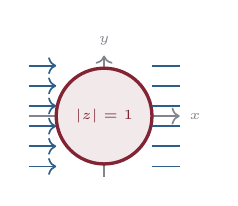
\begin{tikzpicture}[scale=0.64]
          \draw[->, SlateGray!60, line width=0.6pt] (-1.5,0)--(1.5,0) node[right, font=\tiny] {$x$};
          \draw[->, SlateGray!60, line width=0.6pt] (0,-1.2)--(0,1.2) node[above, font=\tiny] {$y$};
          \draw[SapienzaRed, line width=1.2pt, fill=SapienzaRed!10] (0,0) circle (0.95cm);
          \node[font=\tiny\bfseries, text=SapienzaRed] at (0,0) {$|z|=1$};
          \foreach \y in {-1.0,-0.6,-0.2,0.2,0.6,1.0}{
            \draw[AccentBlue, line width=0.6pt, ->] (-1.5,\y) -- (-0.95,\y);
            \draw[AccentBlue, line width=0.6pt] (0.95,\y) -- (1.5,\y);
          }
        \end{tikzpicture}
      \end{center}
  \end{columns}
\end{frame}

\begin{frame}{Isolated Vortex: Critical Core Boundary}
  \chaptag{Ch. 2}
  \begin{columns}[c]
    \column{0.48\textwidth}
      \centering
      \includegraphics[height=0.45\textheight, width=\linewidth, keepaspectratio]%
        {Grafici/Grafici_Particolari/1_FlussoPotenziale_onlyvortex_c0.1.pdf}
      \figcap{Isolated vortex ($n=+1$): circular streamlines and impenetrable normal region boundary at $r=1$.}
    \column{0.48\textwidth}
      \begin{infobox}[Physical Boundary Conditions]
        For an isolated, unpinned vortex at equilibrium:
        \begin{enumerate}
          \item \textbf{Normal Region Boundary ($\mathbf{J}_\perp=0$):}\\
          Supercurrent cannot penetrate the normal region ($\psi=0$ on $|z|=1$).
          \item \textbf{Critical Threshold Equality ($|\mathbf{v}|=1$):}\\
          The physical boundary of the normal region coincides precisely with the critical isoline.
        \end{enumerate}
      \end{infobox}
      \vspace{1pt}
      \begin{warnbox}[Symmetry Preservation]
        Circular symmetry guarantees $|\mathbf{v}|=1/r=1$ exactly on $|z|=1$. No external current $\implies$ exact self-consistency.
      \end{warnbox}
  \end{columns}
\end{frame}

\begin{frame}{Circular Defect in Uniform Flow}
  \chaptag{Ch. 2}
  \begin{columns}[c]
    \column{0.51\textwidth}
      \begin{infobox}[Superposition \& Milne-Thomson Theorem]
        By leveraging the principle of linear superposition and the Milne-Thomson circle theorem, we can model circular defects. An external uniform current is represented by:
        \[f_\mathrm{ext}(z)=ij_0 z\]
      \end{infobox}
      \vspace{1pt}
      \begin{keybox}[Application to the Unit Defect]
        The function representing the current around the defect of radius $r_0=1$ reads:
        \[f(z) = ij_0\!\left(z + \frac{1}{z}\right)\]
        On $|z|=1$, the stream function $\psi = \mathrm{Re}(f) = 0$. This mathematically enforces the physical boundary condition that superconducting Cooper pairs cannot flow into the normal region ($\mathbf{J}_\perp = 0$).
      \end{keybox}
    \column{0.47\textwidth}
      \centering
      \includegraphics[height=0.45\textheight, width=\linewidth, keepaspectratio]%
        {Grafici/Grafici_Particolari/1_FlussoPotenziale_onlyhole_c0.1.pdf}
      \figcap{Uniform flow ($j_0=0.1$) deflected around a rigid circular obstacle.}
  \end{columns}
\end{frame}

% ===========================================================
\sectionframe{3}{Single Vortex}{Zeroth-order model \& geometric feedback}
\section{Chapter 3}
% ===========================================================

\begin{frame}{Fundamental Building Blocks: Superposition}
  \chaptag{Ch. 2}
  \begin{columns}[c]
    \column{0.51\textwidth}
      \begin{infobox}[Three Elementary Analytical Solutions]
        \begin{enumerate}
          \item \textbf{Isolated Vortex ($n=+1$):} $f_\mathrm{v}(z)=\log z,\; W_\mathrm{v}(z)=1/z$.
          \item \textbf{Uniform Current + Circular Hole:}
          $f_\mathrm{h}(z)=ij_0(z+1/z),\; W_\mathrm{h}(z)=ij_0(1-1/z^2)$.
          \item \textbf{Vortex Pinned in External Current:}
          $f(z)=ij_0(z+1/z)+\log z$.
        \end{enumerate}
      \end{infobox}
      \vspace{1pt}
      \begin{warnbox}[The Self-Consistency Challenge]
        When $j_0\neq 0$, the critical isoline $|\mathbf{v}|=1$ detaches from $|z|=1$. Chapter 3 resolves this geometric mismatch via feedback.
      \end{warnbox}
    \column{0.47\textwidth}
      \centering
      \includegraphics[height=0.45\textheight, width=\linewidth, keepaspectratio]%
        {Grafici/Grafici_Particolari/1_FlussoPotenziale_complete_c0.1.pdf}
      \figcap{Linear superposition: pinned vortex driven by uniform supercurrent ($j_0=0.1$). Critical isoline in red dashed.}
  \end{columns}
\end{frame}

\begin{frame}{$0^\mathrm{th}$-Order Baseline: Velocity Asymmetry}
  \chaptag{Ch. 3}
  \begin{columns}[c]
    \column{0.50\textwidth}
      \begin{infobox}[Unperturbed Model ($r_0=1$, fixed at origin)]
        Baseline complex velocity around a rigid unit circle:
        \[W(z)=ij_0\!\left(1-\frac{1}{z^2}\right)+\frac{1}{z}\]
      \end{infobox}
      \vspace{1pt}
      \begin{keybox}[Constructive vs.\ Destructive Superposition]
        For $+j_0$ (rightward flow around counter-clockwise vortex):
        \begin{itemize}
          \item \textbf{South ($y<0$):} External flow and circulation align $\implies |\mathbf{v}|$ is strongly amplified ($|\mathbf{v}| > 1$).
          \item \textbf{North ($y>0$):} External flow and circulation oppose $\implies |\mathbf{v}|$ is suppressed ($|\mathbf{v}| < 1$).
          \item \textbf{Consequence:} The critical isoline $|\mathbf{v}|=1$ deforms and shifts downward relative to the rigid circle.
        \end{itemize}
      \end{keybox}
    \column{0.48\textwidth}
      \centering
      \includegraphics[height=0.45\textheight, width=\linewidth, keepaspectratio]%
        {Grafici/Grafici_Particolari/3_Gradiente_complete_c0.1.pdf}
      \figcap{Velocity gradient field ($j_0=0.1$): strong velocity enhancement at the southern edge, suppression at the north.}
  \end{columns}
\end{frame}

\begin{frame}{Breakdown of Self-Consistency ($0^\mathrm{th}$ Order)}
  \chaptag{Ch. 3}
  \begin{columns}[c]
    \column{0.48\textwidth}
      \centering
      \includegraphics[width=0.82\linewidth, keepaspectratio]%
        {Grafici/Grafici_Generici/maxminY_pre_coords.pdf}
      \figcap{Extremal vertical coordinates ($y_\mathrm{max}, y_\mathrm{min}$) of the critical isoline vs.\ transport current $j_0$.}
    \column{0.50\textwidth}
      \begin{warnbox}[Non-Self-Consistent Boundary]
        Because $|\mathbf{v}|=1$ (dashed red line) detaches from the unit circle (solid black), the model violates boundary self-consistency: the normal region ($\mathbf{J}_\perp=0$) no longer matches the physical critical boundary ($|\mathbf{v}|=1$).
      \end{warnbox}
      \vspace{1pt}
      \begin{infobox}[Vertical Deformation Behavior]
        As transport current $|j_0|$ increases:
        \begin{itemize}
          \item \textbf{Upward Expansion ($y_\mathrm{max}$):} Grows linearly due to velocity suppression above the core.
          \item \textbf{Downward Shift ($y_\mathrm{min}$):} Plunges southward due to strong constructive enhancement.
          \item \textbf{Sharp Inflection:} A slope discontinuity appears at $|j_0|\approx 0.207$.
        \end{itemize}
      \end{infobox}
  \end{columns}
\end{frame}

\begin{frame}{Anisotropic Deformation Across Core}
  \chaptag{Ch. 3}
  \begin{columns}[c]
    \column{0.48\textwidth}
      \centering
      \includegraphics[width=0.82\linewidth, keepaspectratio]%
        {Grafici/Grafici_Generici/maxminX_traslato_pre_coords.pdf}
      \figcap{Horizontal coordinates across the core center ($x_\mathrm{max}, x_\mathrm{min}$) relative to shifted core center.}
    \column{0.50\textwidth}
      \begin{infobox}[Horizontal Rigidity vs.\ Vertical Stretch]
        \begin{itemize}
          \item While vertical stretching across the $y$-axis is severe, the horizontal diameter across the center ($x_\mathrm{max}-x_\mathrm{min}$) remains remarkably rigid.
          \item \textbf{Geometric Anisotropy:} The critical isoline does not expand uniformly as a circle, but stretches anisotropically.
        \end{itemize}
      \end{infobox}
      \vspace{1pt}
      \begin{keybox}[Significance of the Kink at $|j_0|\approx 0.207$]
        A sharp kink appears simultaneously in both horizontal and vertical profiles near $|j_0|\approx 0.207$, indicating a topological transition in isoline curvature. Shifting a rigid circular core must account for this boundary distortion.
      \end{keybox}
  \end{columns}
\end{frame}

\begin{frame}{Origin of the Topological Kink ($|j_0|\approx 0.207$)}
  \chaptag{Ch. 3}
  \begin{columns}[c]
    \column{0.54\textwidth}
      \begin{infobox}[Analytic Evaluation Along $z=iy$]
        Complex velocity along imaginary axis ($z=iy$):
        $W(iy) = i(j_0 y^2 - y + j_0)/y^2 \implies |W(iy)|^2=1$.\\
        Factoring as a difference of squares yields two quadratics:
        $[(j_0-1)y^2 - y + j_0]\cdot[(j_0+1)y^2 - y + j_0]=0$.
      \end{infobox}
      \vspace{1pt}
      \begin{keybox}[Algebraic Root Regimes]
        \begin{itemize}
          \item \textbf{4 Real Roots ($|j_0| \le \frac{-1+\sqrt{2}}{2} \approx 0.207$):}\\
          Both discriminants positive $\implies$ four intersections on $y$-axis (smoothly rounded top).
          \item \textbf{2 Real Roots ($0.207 < |j_0| \le 1.0$):}\\
          One discriminant negative $\implies$ two real roots remain, forming an inward pinching inflection (kink).
        \end{itemize}
      \end{keybox}
    \column{0.44\textwidth}
      \centering
      \vspace{1pt}
      \includegraphics[height=0.45\textheight, width=\linewidth, keepaspectratio]%
        {Grafici/Grafici_Particolari/1_FlussoPotenziale_crit_c0.21.pdf}
      \figcap{Inward pinching inflection: zoomed upper region ($y\approx 1$) showing the critical isoline curving inward toward the core as $j_0$ exceeds $0.207$.}
  \end{columns}
\end{frame}

\begin{frame}{$1^\mathrm{st}$-Order Geometric Feedback: Shift Strategy}
  \chaptag{Ch. 3}
  \begin{columns}[c]
    \column{0.50\textwidth}
      \begin{infobox}[Adapted $1^\mathrm{st}$-Order Potential]
        To mitigate non-self-consistency, we apply a spatial shift $d$ to the rigid circular core along the $y$-axis, aligning it with the deformed critical isoline while keeping the vortex singularity fixed at $z=0$:
        \[f_\mathrm{new}(z)=ij_0\!\left(z+\frac{1}{z-d}\right)+\log z\]
      \end{infobox}
      \vspace{1pt}
      \begin{keybox}[Three Shift Criteria Evaluated]
        \begin{enumerate}
          \item \textbf{1/2 Midpoint Model:} $d = \frac{y_\mathrm{max} + y_\mathrm{min}}{2}$\\
          Centers the core at the exact midpoint of the critical isoline.
          \item \textbf{1/4 Conservative Model:} $d = \frac{y_\mathrm{max} + y_\mathrm{min}}{4}$\\
          Conservative shift half-way toward the isoline midpoint.
          \item \textbf{Extremal Model:} $d = y_\mathrm{min} + 1$ ($j_0\ge 0$)\\
          Aligns lower core edge precisely with the bottom of $|\mathbf{v}|=1$.
        \end{enumerate}
      \end{keybox}
    \column{0.48\textwidth}
      \centering
      \includegraphics[width=0.82\linewidth, keepaspectratio]%
        {Grafici/Grafici_Generici/maxminY_post_coords.pdf}
      \figcap{Vertical coordinates post-feedback: dramatic realignment with the critical isoline boundary.}
  \end{columns}
\end{frame}

\begin{frame}{Geometric Feedback: Horizontal Coordinates}
  \chaptag{Ch. 3}
  \begin{columns}[c]
    \column{0.48\textwidth}
      \centering
      \includegraphics[width=0.82\linewidth, keepaspectratio]%
        {Grafici/Grafici_Generici/maxminX_traslato_post_coords.pdf}
      \figcap{Horizontal coordinates post-feedback relative to shifted core center across all models.}
    \column{0.50\textwidth}
      \begin{infobox}[The Vertical-Horizontal Trade-Off]
        \begin{itemize}
          \item Shifting the core vertically ($y$-axis) eliminates the massive $0^\mathrm{th}$-order vertical mismatch ($y_\mathrm{min}$ and $y_\mathrm{max}$ alignment).
          \item However, because the true isoline stretches anisotropically, shifting a rigid circle slightly perturbs horizontal alignment across the core center ($x_\mathrm{max}, x_\mathrm{min}$).
          \item \textbf{Net Result:} $1^\mathrm{st}$-order feedback provides an immense global improvement in boundary self-consistency across weak and moderate currents.
        \end{itemize}
      \end{infobox}
  \end{columns}
\end{frame}

\begin{frame}{Single Vortex: Strict Transport Reciprocity}
  \chaptag{Ch. 3}
  \begin{columns}[c]
    \column{0.50\textwidth}
      \begin{keybox}[Exact Symmetry Under Reversal]
        The single-vortex configuration is invariant under simultaneous current reversal and spatial reflection across the horizontal axis:
        \[\boxed{j_0 \to -j_0 \quad \Longleftrightarrow \quad y \to -y}\]
        \begin{itemize}
          \item Reversing the current mirrors the velocity field exactly across the $x$-axis.
          \item Consequently, the critical current magnitude required to destroy superconductivity is identical in both directions:
          \[|j_{c,+}| = |j_{c,-}|\]
          \item $\implies$ \textbf{An isolated single vortex exhibits NO macroscopic non-reciprocity or diode effect.}
        \end{itemize}
      \end{keybox}
    \column{0.48\textwidth}
      \begin{infobox}[Low-Current Convergence ($|j_0| < 0.2$)]
        \begin{itemize}
          \item As $j_0\to 0$, all three correction models ($1/2$, $1/4$, and Extremal) converge precisely toward exact self-consistency.
          \item In this weak-current regime, horizontal discrepancies are negligible and results are invariant to the specific correction model chosen.
          \item \textbf{Iterative Pathway:} This strong low-current convergence confirms that applying geometric feedback iteratively converges toward exact self-consistent boundaries.
        \end{itemize}
      \end{infobox}
  \end{columns}
\end{frame}

\begin{frame}{Single Vortex ($j_0=0.1$): Streamlines \& Isolines}
  \chaptag{Ch. 3}
  \begin{columns}[c]
    \column{0.48\textwidth}
      \centering
      \includegraphics[height=0.45\textheight, width=\linewidth, keepaspectratio]%
        {Grafici/Grafici_Particolari/1_FlussoPotenziale_nocorr_c0.1.pdf}
      \figcap{Single Vortex ($j_0=0.1$): Comparison of the complex potential streamlines and isolines around the defect for the $0^\mathrm{th}$ order model.}
    \column{0.48\textwidth}
      \centering
      \includegraphics[height=0.45\textheight, width=\linewidth, keepaspectratio]%
        {Grafici/Grafici_Particolari/1_FlussoPotenziale_corr_noappr_c0.1.pdf}
      \figcap{Single Vortex ($j_0=0.1$): Comparison of the complex potential streamlines and isolines for the 1/2 Feedback Model.}
  \end{columns}
  \vspace{1pt}
  \begin{keybox}[Weak Current Streamline Alignment]
    At $j_0=0.1$, the critical isoline remains nearly circular. The $1^\mathrm{st}$-order shift completely eliminates the boundary mismatch.
  \end{keybox}
\end{frame}

\begin{frame}{Single Vortex ($j_0=0.1$): Surface Velocity Analysis}
  \chaptag{Ch. 3}
  \begin{columns}[c]
    \column{0.48\textwidth}
      \centering
      \includegraphics[width=0.82\linewidth, keepaspectratio]%
        {Grafici/Grafici_Particolari/4_VelocitaBordo_confronto_c0.1.pdf}
      \figcap{Single Vortex ($j_0=0.1$): Combined angular profile of the surface velocity $|\mathbf{v}(\theta)|$ evaluated along the boundary for all models.}
    \column{0.50\textwidth}
      \begin{infobox}[Quantitative Boundary Assessment]
        \begin{itemize}
          \item \textbf{$0^\mathrm{th}$-Order Violation:} Velocity deviates significantly ($|\mathbf{v}| \in [0.8,\, 1.2]$).
          \item \textbf{Optimal Realignment:} $1/2$ and Extremal models dampen peaks, restoring $|\mathbf{v}| \approx 1$.
          \item \textbf{Model Comparison:} $1/2$ and Extremal models are indistinguishable; $1/4$ model is slightly less accurate but effective.
        \end{itemize}
      \end{infobox}
  \end{columns}
\end{frame}

\begin{frame}{Single Vortex ($j_0=0.21$): Streamlines \& Kink Realignment}
  \chaptag{Ch. 3}
  \begin{columns}[c]
    \column{0.48\textwidth}
      \centering
      \includegraphics[height=0.45\textheight, width=\linewidth, keepaspectratio]%
        {Grafici/Grafici_Particolari/1_FlussoPotenziale_crit_c0.21.pdf}
      \figcap{Single Vortex ($j_0=0.21$): Comparison of complex potential streamlines and isolines for the $0^\mathrm{th}$ order model.}
    \column{0.48\textwidth}
      \centering
      \includegraphics[height=0.45\textheight, width=\linewidth, keepaspectratio]%
        {Grafici/Grafici_Particolari/1_FlussoPotenziale_corr_mean_crit_c0.21.pdf}
      \figcap{Single Vortex ($j_0=0.21$): Comparison of complex potential streamlines and isolines for the 1/4 Feedback Model.}
  \end{columns}
  \vspace{1pt}
  \begin{keybox}[Onset of Topological Deformation]
    At $j_0=0.21$, crossing the algebraic root threshold ($0.207$) produces an inward curvature inflection at the top of the critical isoline. Shifting a rigid circle requires careful balancing to avoid over-displacing the core.
  \end{keybox}
\end{frame}

\begin{frame}{Single Vortex ($j_0=0.21$): Surface Velocity Analysis}
  \chaptag{Ch. 3}
  \begin{columns}[c]
    \column{0.48\textwidth}
      \centering
      \includegraphics[width=0.82\linewidth, keepaspectratio]%
        {Grafici/Grafici_Particolari/4_VelocitaBordo_confronto_crit_c0.21.pdf}
      \figcap{Single Vortex ($j_0=0.21$): Combined angular profile of the surface velocity $|\mathbf{v}(\theta)|$ evaluated along the boundary for all models.}
    \column{0.50\textwidth}
      \begin{warnbox}[Why Conservative $1/4$ Feedback Excels Here]
        \begin{itemize}
          \item \textbf{Rigid Circle Limitations:} A rigid circle cannot conform simultaneously to an inward-pinched top boundary and an expanded bottom boundary.
          \item \textbf{Over-Correction Risk:} Aggressive shifts ($1/2$ or Extremal) displace the core too far southward, exposing the northern boundary and inadvertently amplifying local velocity peaks.
          \item \textbf{Optimal Realignment:} The conservative $1/4$ model achieves the best local boundary realignment, keeping $|\mathbf{v}|$ closest to unity.
        \end{itemize}
      \end{warnbox}
  \end{columns}
\end{frame}

\begin{frame}{Single Vortex ($j_0=0.6$): Streamlines \& High-Current Breakdown}
  \chaptag{Ch. 3}
  \begin{columns}[c]
    \column{0.48\textwidth}
      \centering
      \includegraphics[height=0.45\textheight, width=\linewidth, keepaspectratio]%
        {Grafici/Grafici_Particolari/1_FlussoPotenziale_crit_c0.6.pdf}
      \figcap{Single Vortex ($j_0=0.6$): Comparison of complex potential streamlines and isolines for the $0^\mathrm{th}$ order model.}
    \column{0.48\textwidth}
      \centering
      \includegraphics[height=0.45\textheight, width=\linewidth, keepaspectratio]%
        {Grafici/Grafici_Particolari/1_FlussoPotenziale_corr_mean_crit_c0.6.pdf}
      \figcap{Single Vortex ($j_0=0.6$): Comparison of complex potential streamlines and isolines for the 1/4 Feedback Model.}
  \end{columns}
  \vspace{1pt}
  \begin{warnbox}[High-Current Regime Topology]
    Deep inside the high-current regime ($j_0=0.6$), the external transport field heavily dominates intrinsic circulation, forcing massive horizontal stretching across the critical velocity boundary.
  \end{warnbox}
\end{frame}

\begin{frame}{Single Vortex ($j_0=0.6$): Surface Velocity Breakdown}
  \chaptag{Ch. 3}
  \begin{columns}[c]
    \column{0.48\textwidth}
      \centering
      \includegraphics[width=0.82\linewidth, keepaspectratio]%
        {Grafici/Grafici_Particolari/4_VelocitaBordo_confronto_crit_c0.6.pdf}
      \figcap{Single Vortex ($j_0=0.6$): Combined angular profile of the surface velocity $|\mathbf{v}(\theta)|$. The large amplitude variations indicate massive boundary mismatch.}
    \column{0.50\textwidth}
      \begin{warnbox}[Fundamental Limitation of Rigid Spatial Shifts]
        \begin{itemize}
          \item \textbf{Severe Non-Linearity:} The $1^\mathrm{st}$-order rigid circular approximation breaks down because shifting a circle along $y$ cannot absorb horizontal stretching ($x_\mathrm{max}-x_\mathrm{min}$).
          \item \textbf{Boundary Violation:} Velocity vectors cross the assumed circular perimeter at large angles across all feedback models.
          \item \textbf{Required Next Steps:} Achieving self-consistency at high currents requires dynamic core expansion $r_0(j_0)$ and higher-order conformal mappings ($w=g(z)$).
        \end{itemize}
      \end{warnbox}
  \end{columns}
\end{frame}

% ===========================================================
\sectionframe{4}{Dipolar Configuration}{Vortex-antivortex pair \& Diode Effect}
\section{Chapter 4}
% ===========================================================

\begin{frame}{Vortex-Antivortex Dipole ($0^\mathrm{th}$ Order Formulation)}
  \chaptag{Ch. 4}
  \begin{columns}[c]
    \column{0.50\textwidth}
      \begin{infobox}[Dipolar Complex Potential ($0^\mathrm{th}$ Order)]
        Bound vortex ($+1$ at $+id/2$) and antivortex ($-1$ at $-id/2$) separated by distance $d$ in uniform flow $j_0$:
        \begin{align*}
          f(z) &= ij_0\!\left(z + \frac{1}{z-i\frac{d}{2}} + \frac{1}{z+i\frac{d}{2}}\right) \\
               &\quad + \log\!\left(z-i\frac{d}{2}\right) - \log\!\left(z+i\frac{d}{2}\right)
        \end{align*}
      \end{infobox}
      \vspace{1pt}
      \begin{keybox}[The Central Superconducting Channel]
        \begin{itemize}
          \item A dissipationless channel separates the two cores across $y=0$.
          \item If critical isolines touch across $y=0$, the channel collapse $\implies$ vortex-antivortex annihilation into a resistive state.
          \item \textit{Linear superposition is exact when $d \gg r_0=1$.}
        \end{itemize}
      \end{keybox}
    \column{0.48\textwidth}
      \centering
      \includegraphics[height=0.45\textheight, width=\linewidth, keepaspectratio]%
        {Grafici/Grafici_Dipolo/1_FlussoPotenziale_linsep_nocorr_c0_dati.pdf}
      \figcap{Dipolar Configuration ($j_0=0, d=8$): Asymmetric current in a vortex-antivortex pair separated by an initial center-to-center distance $d=8$ without external current.}
  \end{columns}
\end{frame}

\begin{frame}{Dipolar Superposition with External Current ($j_0=0.1$)}
  \chaptag{Ch. 4}
  \begin{columns}[c]
    \column{0.48\textwidth}
      \centering
      \includegraphics[height=0.45\textheight, width=\linewidth, keepaspectratio]%
        {Grafici/Grafici_Dipolo/1_FlussoPotenziale_linsep_nocorr_c0.1_dati.pdf}
      \figcap{Streamlines and isolines.}
    \column{0.48\textwidth}
      \centering
      \includegraphics[height=0.45\textheight, width=\linewidth, keepaspectratio]%
        {Grafici/Grafici_Dipolo/3_Gradiente_linsep_nocorr_c0.1_dati.pdf}
      \figcap{Gradient vector field.}
  \end{columns}
\end{frame}

\begin{frame}{Channel Width vs.\ Current ($0^\mathrm{th}$ Order)}
  \chaptag{Ch. 4}
  \begin{columns}[c]
    \column{0.50\textwidth}
      \centering
      \includegraphics[width=0.82\linewidth, keepaspectratio]%
        {Grafici/Grafici_Dipolo/Base_DistanzaLobi1.pdf}
      \figcap{Dipolar Configuration ($0^{\text{th}}$ Order): Vertical channel gap between disjoint isolines vs.\ $j_0$ across initial separations $d$.}
    \column{0.48\textwidth}
      \begin{infobox}[Key Physical Observations]
        \begin{itemize}
          \item Larger $d$: weaker mutual interaction $\implies$ channel persists to higher currents.
          \item $j_0>0$: gap decreases rapidly (constructive amplification $\to$ early collapse).
          \item $j_0<0$: gap decreases very slowly (destructive suppression $\to$ open channel).
          \item Discontinuity at $|j_0|\approx 0.207$: marks the algebraic topological kink.
        \end{itemize}
      \end{infobox}
  \end{columns}
\end{frame}

\begin{frame}{Dipolar Phase Diagram ($0^\mathrm{th}$ Order)}
  \chaptag{Ch. 4}
  \begin{columns}[c]
    \column{0.50\textwidth}
      \centering
      \includegraphics[width=0.82\linewidth, keepaspectratio]%
        {Grafici/Grafici_Dipolo/Fase_Base1.pdf}
      \figcap{Phase diagram mapping transition boundaries between separated and merged critical isolines.}
    \column{0.48\textwidth}
      \begin{keybox}[Stability Thresholds]
        \begin{itemize}
          \item \textbf{Critical Distance ($d^{(0)}_\mathrm{crit} \approx 4$):}\\ Minimum separation for disjoint lobes at $j_0=0$.
          \item \textbf{Dynamic Stabilization:}\\ For $d < 4$, applying a negative current ($j_0 < 0$) can destructively suppress the velocity field sufficiently to re-separate the merged lobes into distinct topological domains.
        \end{itemize}
      \end{keybox}
  \end{columns}
\end{frame}

\begin{frame}{$1^\mathrm{st}$-Order Feedback on the Dipole}
  \chaptag{Ch. 4}
  \begin{columns}[c]
    \column{0.50\textwidth}
      \begin{infobox}[Adapted $1^\mathrm{st}$-Order Dipolar Potential]
        normal regions shift symmetrically to $\pm i\frac{d_\mathrm{new}}{2}$, while topological singularities remain fixed at $\pm i\frac{d}{2}$:
        \begin{align*}
          f_\mathrm{new} &= ij_0\!\left(z + \frac{1}{z-i\frac{d_\mathrm{new}}{2}} + \frac{1}{z+i\frac{d_\mathrm{new}}{2}}\right) \\
                         &\quad + \log\frac{z-i\frac{d}{2}}{z+i\frac{d}{2}}
        \end{align*}
      \end{infobox}
      \vspace{1pt}
      \begin{keybox}[Internal vs.\ Midpoint Feedback Models]
        \begin{itemize}
          \item \textbf{Internal Model:} Shifting based strictly on inner extremal coordinate facing the central channel.
          \item \textbf{Midpoint/Conservative Models:} Shifts cores inward when $j_0>0$, narrowing the gap and accelerating collapse vs.\ baseline ($\implies$ lower $j_{c,+}$).
        \end{itemize}
      \end{keybox}
    \column{0.48\textwidth}
      \centering
      \includegraphics[width=0.82\linewidth, keepaspectratio]%
        {Grafici/Grafici_Dipolo/Unified_Phase_Diagram_Feedback.pdf}
      \figcap{Unified $1^\mathrm{st}$-Order Phase Diagrams: all models agree qualitatively on directional asymmetry.}
  \end{columns}
\end{frame}

\begin{frame}{Dipole Channel Width vs.\ Current ($1^\mathrm{st}$ Order)}
  \chaptag{Ch. 4}
  \begin{columns}[c]
    \column{0.50\textwidth}
      \centering
      \includegraphics[width=0.82\linewidth, keepaspectratio]%
        {Grafici/Grafici_Dipolo/DistanzaLobi_Combined.pdf}
      \figcap{Vertical separation vs $j_0$ comparing baseline to geometric feedback models.}
    \column{0.48\textwidth}
      \begin{infobox}[Channel Gap Dynamics]
        \begin{itemize}
          \item Feedback physically shifts normal regions inward when $j_0>0$, resulting in a smaller channel gap compared to the $0^\mathrm{th}$-order baseline.
          \item \textbf{Model Hierarchy:} Internal feedback dictates the most aggressive shift, triggering the earliest collapse. 1/4 feedback is the most conservative.
        \end{itemize}
      \end{infobox}
  \end{columns}
\end{frame}

\begin{frame}{Unified $1^\mathrm{st}$-Order Dipolar Phase Diagrams}
  \chaptag{Ch. 4}
  \begin{columns}[c]
    \column{0.50\textwidth}
      \centering
      \includegraphics[width=0.82\linewidth, keepaspectratio]%
        {Grafici/Grafici_Dipolo/Unified_Phase_Diagram_Feedback.pdf}
      \figcap{Phase diagrams comparing transition thresholds of all feedback models.}
    \column{0.48\textwidth}
      \begin{keybox}[Robustness of Phase Boundaries]
        \begin{itemize}
          \item The system is significantly more susceptible to channel collapse than predicted by the rigid baseline.
          \item \textbf{Directional Asymmetry:} The macroscopic critical threshold depends strictly on the current sign.
        \end{itemize}
      \end{keybox}
  \end{columns}
\end{frame}

\begin{frame}{Macroscopic Dipolar Non-Reciprocity: Gradient Fields}
  \chaptag{Ch. 4}
  \begin{columns}[c]
    \column{0.48\textwidth}
      \centering
      \includegraphics[height=0.45\textheight, width=\linewidth, keepaspectratio]%
        {Grafici/Grafici_Dipolo/3_Gradiente_linsep_nocorr_c-0.5_dati.pdf}
      \figcap{Superconducting Diode Effect ($d=8$): Comparison of the current gradient vector fields under external current $j_1=-0.5$ in the $0^{\text{th}}$ order model.}
    \column{0.48\textwidth}
      \centering
      \includegraphics[height=0.45\textheight, width=\linewidth, keepaspectratio]%
        {Grafici/Grafici_Dipolo/3_Gradiente_linsep_nocorr_c0.5_dati.pdf}
      \figcap{Superconducting Diode Effect ($d=8$): Comparison of the current gradient vector fields under external current $j_2=0.5$ in the $0^{\text{th}}$ order model.}
  \end{columns}
  \vspace{1pt}
  \begin{keybox}[Breaking of Spatial Inversion Symmetry]
    Because the dipole breaks vertical symmetry along $y$, current direction strictly controls interference in the central channel. Transport is \textbf{strongly non-reciprocal}: supercurrent flows dissipationlessly in one direction but collapses the gap in the other.
  \end{keybox}
\end{frame}

\begin{frame}{Superconducting Diode Effect: Surface Velocity Analysis}
  \chaptag{Ch. 4}
  \begin{columns}[c]
    \column{0.48\textwidth}
      \centering
      \includegraphics[width=0.82\linewidth, keepaspectratio]%
        {Grafici/Grafici_Dipolo/4_VelocitaBordo_linsep_nocorr_c-0.5_dati.pdf}
      \figcap{Superconducting Diode Effect ($d=8$): Comparison of the surface velocity along the boundary of the lower normal region under external current $j_1=-0.5$.}
    \column{0.48\textwidth}
      \centering
      \includegraphics[width=0.82\linewidth, keepaspectratio]%
        {Grafici/Grafici_Dipolo/4_VelocitaBordo_linsep_nocorr_c0.5_dati.pdf}
      \figcap{Superconducting Diode Effect ($d=8$): Comparison of the surface velocity along the boundary of the lower normal region under external current $j_2=0.5$.}
  \end{columns}
  \vspace{1pt}
  \begin{keybox}[Direction-Dependent Critical Threshold ($\boxed{j_{c,+}\; \ll \; |j_{c,-}|}$)]
    For any transport current $j_0 \in (j_{c,+},\, |j_{c,-}|)$, forward flow ($+j_0$) collapses the channel into a resistive state while reverse flow ($-j_0$) conducts dissipationlessly. Pinned topological defects inherently induce a Superconducting Diode Effect.
  \end{keybox}
\end{frame}

\begin{frame}{Dipolar ($j_0=-0.5, d=8$): Streamline Topology}
  \chaptag{Ch. 4}
  \begin{columns}[c]
    \column{0.48\textwidth}
      \centering
      \includegraphics[height=0.45\textheight, width=\linewidth, keepaspectratio]%
        {Grafici/Grafici_Dipolo/1_FlussoPotenziale_linsep_nocorr_c-0.5_dati.pdf}
      \figcap{Dipolar Configuration ($j_0=-0.5, d=8$): Application of the $0^\mathrm{th}$ Order model under a strong negative transport current.}
    \column{0.48\textwidth}
      \centering
      \includegraphics[height=0.45\textheight, width=\linewidth, keepaspectratio]%
        {Grafici/Grafici_Dipolo/1_FlussoPotenziale_linsep_corrfor_c-0.5_dati.pdf}
      \figcap{Dipolar Configuration ($j_0=-0.5, d=8$): Application of the 1/2 Feedback model under a strong negative transport current.}
  \end{columns}
  \vspace{1pt}
  \begin{keybox}[Strong Negative Current Regime]
    Because the critical isolines remain topologically disjoint under reverse flow ($j_0=-0.5$)â€â€Âunlike the macroscopic merging at $j_0=+0.5$---the independent two-circle assumption remains valid, allowing geometric feedback to operate safely.
  \end{keybox}
\end{frame}

\begin{frame}{Dipolar ($j_0=-0.5, d=8$): Surface Velocity Profile}
  \chaptag{Ch. 4}
  \begin{columns}[c]
    \column{0.48\textwidth}
      \centering
      \includegraphics[width=0.82\linewidth, keepaspectratio]%
        {Grafici/Grafici_Dipolo/4_VelocitaBordo_confronto_c-0.5.pdf}
      \figcap{Dipolar Configuration ($j_0=-0.5, d=8$): Combined angular profile of the surface velocity $|\mathbf{v}(\theta)|$ under strong negative external current.}
    \column{0.50\textwidth}
      \begin{infobox}[Quantitative Boundary Assessment]
        \begin{itemize}
          \item \textbf{$0^\mathrm{th}$-Order Violation:} Unperturbed baseline exhibits substantial velocity fluctuations around the circular boundary due to strong external flow ($|j_0|=0.5$).
          \item \textbf{Feedback Correction:} Implementing $1^\mathrm{st}$-order spatial shifts ($1/4$ and Internal) measurably improves boundary self-consistency toward $|\mathbf{v}|\approx 1$.
          \item \textbf{Strong-Drive Limit:} While measurable improvements occur, $|j_0|=0.5$ represents a strong drive where residual fluctuations persist.
        \end{itemize}
      \end{infobox}
  \end{columns}
\end{frame}

\begin{frame}{Dipolar ($j_0=0.1, d=8$): Streamline Alignment}
  \chaptag{Ch. 4}
  \begin{columns}[c]
    \column{0.48\textwidth}
      \centering
      \includegraphics[height=0.45\textheight, width=\linewidth, keepaspectratio]%
        {Grafici/Grafici_Dipolo/1_FlussoPotenziale_linsep_nocorr_c0.1_dati.pdf}
      \figcap{Dipolar Configuration ($j_0=0.1, d=8$): Application of the $0^\mathrm{th}$ Order baseline model.}
    \column{0.48\textwidth}
      \centering
      \includegraphics[height=0.45\textheight, width=\linewidth, keepaspectratio]%
        {Grafici/Grafici_Dipolo/1_FlussoPotenziale_linsep_corrmed_c0.1_dati.pdf}
      \figcap{Dipolar Configuration ($j_0=0.1, d=8$): Application of the 1/4 Feedback model, demonstrating the spatial shift of the physical normal regions.}
  \end{columns}
  \vspace{1pt}
  \begin{keybox}[Weak Forward Current Regime]
    At weak positive current ($j_0=0.1$), the critical isolines are widely separated across the central channel ($d=8$). All three geometric feedback models prove highly effective at mitigating boundary non-self-consistency.
  \end{keybox}
\end{frame}

\begin{frame}{Dipolar ($j_0=0.1, d=8$): Surface Velocity Assessment}
  \chaptag{Ch. 4}
  \begin{columns}[c]
    \column{0.48\textwidth}
      \centering
      \includegraphics[width=0.82\linewidth, keepaspectratio]%
        {Grafici/Grafici_Dipolo/4_VelocitaBordo_confronto_c0.1.pdf}
      \figcap{Dipolar Configuration ($j_0=0.1, d=8$): Combined angular profile of the surface velocity $|\mathbf{v}(\theta)|$ evaluating the boundary alignment for all models.}
    \column{0.50\textwidth}
      \begin{infobox}[Optimal Low-Current Realignment]
        \begin{itemize}
          \item \textbf{Remarkable Convergence:} All feedback methods ($1/2$, $1/4$, Internal) eliminate $0^\mathrm{th}$-order velocity variations, restoring $|\mathbf{v}|\approx 1$ uniformly.
          \item \textbf{Subtle Distinction:} The Internal model shows slightly larger residual velocity fluctuations along the core perimeter compared to $1/2$ and $1/4$.
          \item \textbf{Global Agreement:} Macroscopic streamlines and supercurrent deflections across the channel are indistinguishable among all three models.
        \end{itemize}
      \end{infobox}
  \end{columns}
\end{frame}

\begin{frame}{Dipole --- Feedback at $j_0=0.1$ ($d=8$)}
  \chaptag{Ch. 4}
  \begin{columns}[t]
    \column{0.48\textwidth}
      \centering
      \includegraphics[height=0.65\textheight, width=\linewidth, keepaspectratio]%
        {Grafici/Grafici_Dipolo/1_FlussoPotenziale_linsep_corrmed_c0.1_dati.pdf}
      \figcap{1/4 Feedback Model.}
    \column{0.48\textwidth}
      \centering
      \includegraphics[height=0.65\textheight, width=\linewidth, keepaspectratio]%
        {Grafici/Grafici_Dipolo/4_VelocitaBordo_confronto_c0.1.pdf}
      \figcap{Surface velocity $|\mathbf{v}(\theta)|$ comparison.}
  \end{columns}
  \vspace{10pt}
  \figcap{Dipolar Configuration ($j_0=0.1, d=8$): Application of the feedback models compared to the unperturbed baseline, demonstrating the spatial shift of the physical normal regions.}
\end{frame}

\begin{frame}{Dipolar ($j_0=0.4, d=8$): Streamlines Near Threshold}
  \chaptag{Ch. 4}
  \begin{columns}[t]
    \column{0.48\textwidth}
      \centering
      \includegraphics[height=0.65\textheight, width=\linewidth, keepaspectratio]%
        {Grafici/Grafici_Dipolo/1_FlussoPotenziale_linsep_nocorr_c0.4_dati.pdf}
      \figcap{$0^\mathrm{th}$ Order Model.}
    \column{0.48\textwidth}
      \centering
      \includegraphics[height=0.65\textheight, width=\linewidth, keepaspectratio]%
        {Grafici/Grafici_Dipolo/1_FlussoPotenziale_linsep_corrmed_c0.4_dati.pdf}
      \figcap{1/4 Feedback Model.}
  \end{columns}
  \vspace{10pt}
  \figcap{Dipolar Configuration ($j_0=0.4, d=8$): Application of the feedback models compared to the unperturbed baseline, demonstrating the spatial shift of the physical normal regions.}
\end{frame}

\begin{frame}{Dipolar ($j_0=0.4, d=8$): Surface Velocity \& Breakdown}
  \chaptag{Ch. 4}
  \begin{columns}[c]
    \column{0.48\textwidth}
      \centering
      \includegraphics[width=0.82\linewidth, keepaspectratio]%
        {Grafici/Grafici_Dipolo/4_VelocitaBordo_confronto_c0.4.pdf}
      \figcap{Dipolar Configuration ($j_0=0.4, d=8$): Combined angular profile of the surface velocity $|\mathbf{v}(\theta)|$ under high external current.}
    \column{0.50\textwidth}
      \begin{warnbox}[Why Aggressive Shifts Fail Near Threshold]
        \begin{itemize}
          \item \textbf{Premature Collision:} Shifting cores inward via aggressive models ($1/2$ or Internal) forces physical circles to collide prematurely across $y=0$, causing unphysical channel collapse.
          \item \textbf{Conservative Superiority:} The $1/4$ model performs best because its conservative displacement preserves open channel topology while mitigating boundary velocity peaks.
          \item \textbf{Two-Circle Limit:} Demonstrates that rigid circle shifts must give way to dynamic shape deformations when isolines stretch near critical thresholds.
        \end{itemize}
      \end{warnbox}
  \end{columns}
\end{frame}

\begin{frame}{Dipole Near Threshold ($j_0=0.4, d=8$)}
  \chaptag{Ch. 4}
  \begin{columns}[t]
    \column{0.48\textwidth}
      \centering
      \includegraphics[height=0.65\textheight, width=\linewidth, keepaspectratio]%
        {Grafici/Grafici_Dipolo/1_FlussoPotenziale_linsep_nocorr_c0.4_dati.pdf}
      \figcap{$0^\mathrm{th}$ Order Model.}
    \column{0.48\textwidth}
      \centering
      \includegraphics[height=0.65\textheight, width=\linewidth, keepaspectratio]%
        {Grafici/Grafici_Dipolo/1_FlussoPotenziale_linsep_corrmed_c0.4_dati.pdf}
      \figcap{1/4 Feedback Model.}
  \end{columns}
  \vspace{10pt}
  \figcap{Dipolar Configuration ($j_0=0.4, d=8$): The 1/4 Model preserves disjoint topology, preventing premature channel collapse seen in the baseline model.}
\end{frame}

% ===========================================================
\section{Conclusions}
% ===========================================================

\begin{frame}{Conclusions: Methodology \& Single Pinned Vortex}
  \begin{columns}[c]
    \column{0.50\textwidth}
      \begin{keybox}[Methodological \& Single-Vortex Synthesis]
        \begin{enumerate}
          \item \textbf{Conformal Mapping for Superfluids:}\\
          Because macroscopic phase obeys Laplace's equation ($\nabla^2\theta=0$), conformal mapping provides an exact analytical framework for modeling 2D superfluid velocity around boundaries.
          \item \textbf{Boundary Realignment:}\\
          First-order geometric feedback successfully realigns normal regions with deformed critical isolines across weakly driven regimes ($|j_0|<0.2$).
          \item \textbf{Strict Single-Vortex Reciprocity:}\\
          Isolated vortices obey exact current reversal symmetry ($j_0 \to -j_0 \Leftrightarrow y \to -y$), yielding strictly reciprocal transport ($|j_{c,+}| = |j_{c,-}|$).
        \end{enumerate}
      \end{keybox}
    \column{0.48\textwidth}
      \centering
      \includegraphics[height=0.45\textheight, width=\linewidth, keepaspectratio]%
        {Grafici/Grafici_Particolari/1_FlussoPotenziale_corr_noappr_c0.1.pdf}
      \figcap{Single vortex feedback ($j_0=0.1$): exact boundary self-consistency and spatial reflection symmetry.}
  \end{columns}
\end{frame}

\begin{frame}{Conclusions: Dipolar Non-Reciprocity \& Diode Effect}
  \begin{columns}[c]
    \column{0.50\textwidth}
      \begin{keybox}[Dipolar Diode Synthesis]
        \begin{enumerate}
          \item \textbf{Broken Spatial Symmetry:}\\
          Interacting vortex-antivortex pairs break spatial inversion along $y$. Constructive vs.\ destructive interference strictly dictates directional channel stability.
          \item \textbf{Superconducting Diode Effect:}\\
          Directional channel collapse establishes a robust critical threshold gap ($\boxed{j_{c,+} \ll |j_{c,-}|}$), enabling dissipationless forward blocking and reverse conduction.
          \item \textbf{Robustness Across Models:}\\
          While specific shift criteria ($1/2$, $1/4$, Internal) vary near threshold, all models agree on the phase diagram structure and directional diode property.
        \end{enumerate}
      \end{keybox}
    \column{0.48\textwidth}
      \centering
      \includegraphics[width=0.82\linewidth, keepaspectratio]%
        {Grafici/Grafici_Dipolo/Unified_Phase_Diagram_Feedback.pdf}
      \figcap{Unified phase boundaries: directional non-reciprocity is a robust physical property across all approximations.}
  \end{columns}
\end{frame}

\begin{frame}{Future Perspectives \& Analytical Refinements}
  \begin{columns}[c]
    \column{0.50\textwidth}
      \begin{infobox}[Methodological Refinements]
        \begin{itemize}
          \item \textbf{Iterative Self-Consistent Loop:} Transition from single-step feedback to automated iterations. For $|j_0|<0.2$, this converges mathematically to exact self-consistent boundaries.
          \item \textbf{Dynamic Core Expansion $r_0(j_0)$:} Overcome rigid-circle limits by allowing effective core radius to expand/shrink with local supercurrent density.
          \item \textbf{Higher-Order Conformal Mappings:} Map the unit circle onto elliptical profiles to exactly match high-current ($|j_0|\ge 0.4$) isoline stretching.
        \end{itemize}
      \end{infobox}
    \column{0.48\textwidth}
      \begin{keybox}[Experimental Transport Devices]
        \begin{itemize}
          \item \textbf{Bridging the Gap:} Capturing exact morphological deformations bridges the gap between idealized potential flow theory and the pronounced non-reciprocity of the superconducting diode effect.
          \item \textbf{Quantitative Comparisons:} This advancement will allow for direct, quantitative comparisons with modern experimental transport devices.
        \end{itemize}
      \end{keybox}
      \vspace{2pt}
      \begin{center}
        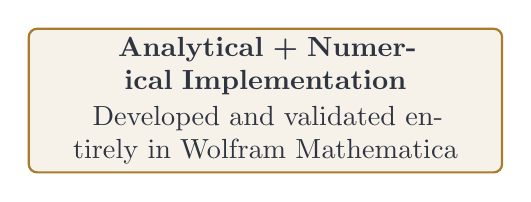
\begin{tikzpicture}
          \node[draw=SapienzaGold, line width=0.8pt, rounded corners=3pt,
                fill=SapienzaGold!10, text width=5.8cm, align=center,
                inner sep=3pt, font=, text=SlateGray] {
            \textbf{Analytical + Numerical Implementation}\\[1pt]
            Developed and validated entirely in Wolfram Mathematica
          };
        \end{tikzpicture}
      \end{center}
  \end{columns}
\end{frame}

% ---- THANK YOU ----
{\setbeamertemplate{footline}{}
\begin{frame}[plain]
  \begin{tikzpicture}[remember picture, overlay]
    \fill[SapienzaRed]
      (current page.north west) rectangle (current page.south east);
    \fill[SapienzaGold, opacity=0.22]
      ([xshift=6cm, yshift=-1cm]current page.center) circle (6cm);
    \fill[SapienzaGold]
      (current page.north west) rectangle
      ([xshift=0.4cm]current page.south west);
    \node[text=white, font=\fontsize{40}{40}\bfseries\selectfont]
      at ([xshift=0.2cm]current page.center) {Thank You};
    \node[text=white!65, font=\large\itshape, yshift=-1.4cm]
      at ([xshift=0.2cm]current page.center) {Questions \& Discussion};
    \draw[white!30, line width=0.5pt]
      ([xshift=-4.5cm, yshift=-2.1cm]current page.center) --
      ([xshift=4.5cm, yshift=-2.1cm]current page.center);
    \node[text=white!50, font=\small, yshift=-2.6cm]
      at ([xshift=0.2cm]current page.center)
      {Francesco Lupicuti \;\textbullet\;
       Sapienza Universit\`a di Roma \;\textbullet\; July 2026};
  \end{tikzpicture}
\end{frame}}

% ===========================================================
\begin{frame}[allowframebreaks]{References}
  \begin{thebibliography}{99}
    \setbeamertemplate{bibliography item}[text]
    \fontsize{7.5}{9}\selectfont
    
    \bibitem{ginzburg1965theory}
    V.~L. Ginzburg and L.~D. Landau.
    \newblock \emph{On the theory of superconductivity}.
    \newblock Collected Papers of L.D. Landau, 546--568 (1965).

    \bibitem{bardeen1957theory}
    J.~Bardeen, L.~N. Cooper, and J.~R. Schrieffer.
    \newblock \emph{Theory of superconductivity}.
    \newblock Phys. Rev. \textbf{108}, 1175 (1957).
    
    \bibitem{cooper1956bound}
    L.~N. Cooper.
    \newblock \emph{Bound electron pairs in a degenerate Fermi gas}.
    \newblock Phys. Rev. \textbf{104}, 1189 (1956).

    \bibitem{chaikin1995principles}
    P.~M. Chaikin and T.~C. Lubensky.
    \newblock \emph{Principles of condensed matter physics}.
    \newblock Cambridge University Press (1995).

    \bibitem{milne1968theoretical}
    L.~M. Milne-Thomson.
    \newblock \emph{Theoretical hydrodynamics}.
    \newblock Dover Publications (1968).

    \bibitem{ando2020observation}
    F. Ando et al.
    \newblock \emph{Observation of superconducting diode effect}.
    \newblock Nature \textbf{584}, 373--376 (2020).

    \bibitem{mermin1966absence}
    N.~D. Mermin and H.~Wagner.
    \newblock \emph{Absence of Ferromagnetism or Antiferromagnetism in One- or Two-Dimensional Isotropic Heisenberg Models}.
    \newblock Phys. Rev. Lett. \textbf{17}, 1133 (1966).

    \bibitem{kosterlitz1973ordering}
    J.~M. Kosterlitz and D.~J. Thouless.
    \newblock \emph{Ordering, metastability and phase transitions in two-dimensional systems}.
    \newblock J. Phys. C: Solid State Phys. \textbf{6}, 1181 (1973).

    \bibitem{berezinskii1971destruction}
    V.~L. Berezinskii.
    \newblock \emph{Destruction of long-range order in one-dimensional and two-dimensional systems having a continuous symmetry group I. Classical systems}.
    \newblock Sov. Phys. JETP \textbf{32}, 493 (1971).

    \bibitem{berezinskii1972destruction}
    V.~L. Berezinskii.
    \newblock \emph{Destruction of long-range order in one-dimensional and two-dimensional systems having a continuous symmetry group II. Quantum systems}.
    \newblock Sov. Phys. JETP \textbf{34}, 610 (1972).

    \bibitem{daido2022intrinsic}
    A.~Daido, Y.~Ikeda, and Y.~Yanase.
    \newblock \emph{Intrinsic superconducting diode effect}.
    \newblock Phys. Rev. Lett. \textbf{128}, 037001 (2022).

    \bibitem{brown2013complex}
    J.~W. Brown and R.~V. Churchill.
    \newblock \emph{Complex Variables and Applications}.
    \newblock McGraw-Hill Education (2013).

    \bibitem{clem2011geometry}
    J.~R. Clem and K.~K. Berggren.
    \newblock \emph{Geometry-dependent critical currents in superconducting nanocircuits}.
    \newblock Phys. Rev. B \textbf{84}, 174510 (2011).

    \bibitem{kogan2014manipulating}
    V.~G. Kogan and R.~G. Mints.
    \newblock \emph{Manipulating Josephson junctions in thin-films by nearby vortices}.
    \newblock Physica C \textbf{502}, 58--62 (2014).

    \bibitem{tinkham1996introduction}
    M.~Tinkham.
    \newblock \emph{Introduction to Superconductivity}.
    \newblock McGraw-Hill (1996).

    \bibitem{martin1997artificial}
    J.~I. Mart{\'\i}n et al.
    \newblock \emph{Artificial flux pinning with magnetic dots}.
    \newblock Phys. Rev. Lett. \textbf{79}, 1929 (1997).
  \end{thebibliography}
\end{frame}

% ===========================================================
\appendix
\end{document}
























